% vim: set tw=78 tabstop=4 shiftwidth=4 aw ai:

\chapter{Protocol Measurement and Analysis in Peer-to-Peer Systems}
\label{chapter:proto-measure}

We undertook a novel approach involving client-side information collection
regarding client and protocol implementation. We have instrumented a
libtorrent-rasterbar
client\footnote{\url{http://www.rasterbar.com/products/libtorrent/}} and a
Tribler\footnote{\url{http://www.tribler.org/trac/}} client to provide verbose
information regarding BitTorrent protocol implementation. These results are
collected and subsequently processed and analysed through a rendering
interface.

Our aim is to measure and analyze protocol messages while in real-world
environments. As described in Chapter~\ref{chapter:virt-infra}, a virtualized
infrastructure had been used for realistic environments; apart from that,
clients and trackers running in a real-world swarm have been used and
instrumented to provide valuable protocol information and parameters. No
simulators have been used for collecting, measuring and analyzing protocol
parameters, rather a ``keep it real as much as possible'' approach.
Information, messages and parameters are collected directly from peers and
trackers that are part of a real-world Peer-to-Peer swarm. Simulator
approaches may reach a complete simulation of the BitTorrent in a network
emulator (OMNet++)~\cite{simulating-bittorrent}.

\section{BitTorrent Messages and Parameters}
\label{sec:proto-measure:protocol-messages}

Analysis of BitTorrent client-centric behavior and, to some extent, swarm
behavior, is based on BitTorrent protocol
messages\footnote{\url{http://www.bittorrent.org/beps/bep\_0003.html}}. Messages are
used for handshaking, closing the connection, requesting and receiving data.

The BitTorrent client will generate at startup a unique identifier of itself,
known as \textit{peer id}. This is client dependent, each client encoding a
peer id based on its own implementation.

\subsection{Protocol Messages}

Swarm measured data are usually collected from trackers. While this offers a
global view of the swarm it has little information about client-centric
properties such as protocol implementation, neighbour set, number of connected
peers, etc. A more thorough approach has been presented by
Iosup~et~al.~\cite{corr-overlay}, using network probes to interrogate various
clients.  A similar approach had been undertaken by
Zhang~et~al.~\cite{p2p-trace-archive}, who created an online available
Peer-to-Peer trace archive, consisting of information from previous
experiments, and using a diversity of Peer-to-Peer protocols.

Our approach~\cite{enhanced-logging}, while not as scalable as the above
mentioned one, aims to collect client-centric data, store and analyse it in
order to provide information on the impact of network topology, protocol
implementation and peer characteristics. Our infrastructure provides
micro-analysis, rather than macro-analysis of a given swarm. We focus on
detailed peer-centric properties, rather than less-detailed global,
tracker-centric information. The data provided by controlled instrumented
peers in a given swarm is retrieved, parsed and stored for subsequent
analysis.

We differentiate between two kinds of BitTorrent messages: \textit{status
messages}, which clients provide periodically to report the current session’s
download state, and \textit{verbose messages} that contain protocol messages
exchanged between peers (chokes, unchokes, peer connections, pieces transfer
etc.).

Another type of messages are those provided by tracker
logging~\cite{tracker-mon}. Tracker-based
messages provide an overall view of the entire swarm, albeit at the cost of
less-detailed information. Tracker logging typically consists of periodic
messages sent by clients as announce messages. However, these messages' period
is quite large (usually 30 minutes -- 1800 seconds) resulting in less detailed
information. Their overall swarm vision is an important addition to status and
verbose client messages.

\subsection{Measured Data and Parameters}

Data and parameters measured are those particular to BitTorrent clients and
swarms, that provide support for evaluation and improvements at protocol level.
The measured parameters are described in
Table~\ref{tab:proto-measure:status-messages-params},
Table~\ref{tab:proto-measure:verbose-messages-params} and
Table~\ref{tab:proto-measure:tracker-messages-params}, depending
on their source (either status messages, verbose messages or tracker
messages).

\begin{table}[htb]
  \centering
  \caption{Parameters from Status Messages}
  \label{tab:proto-measure:status-messages-params}
  \begin{tabular}{@{}ll@{}}
    \toprule
      \textbf{Parameter} & \textbf{Explanation} \\
    \midrule
      Download speed & Current peer download speed -- number of bytes
      received \\
      Upload speed & Current peer upload speed -- number of bytes sent \\
      ETA & How long before the complete file is received \\
      Number of connections & Number of remote peers currently connected to
      this client \\
      Download size & Bytes download so far \\
      Upload size & Bytes uploaded so far \\
      Remote peers ID & IP address and TCP port of remote peers \\
      Per-remote peer download speed & Download speed of each remote connected
      peer \\
      Per-peer upload speed & Upload speed of each remote connected peer \\
    \bottomrule
  \end{tabular}
\end{table}

\begin{table}[htb]
  \centering
  \caption{Parameters from Verbose Messages}
  \label{tab:proto-measure:verbose-messages-params}
  \begin{tabular}{@{}ll@{}}
    \toprule
      \textbf{Parameter} & \textbf{Explanation} \\
    \midrule
      \texttt{CHOKE} & Disallow remote peer to request pieces \\
      \texttt{UNCHOKE} & Allow remote peer to request pieces \\
      \texttt{INTERESTED} & Mark interest in a certain piece \\
      \texttt{NOT\_INTERESTED} & Unmark interest in a certain piece \\
      \texttt{HAVE} & Remote peer possesses current piece \\
      \texttt{BITFIELD} & Bitmap of the file \\
      \texttt{REQUEST} & Ask for a given piece \\
      \texttt{PIECE} & Send piece \\
      \texttt{CANCEL} & Cancel request of a piece \\
      \texttt{DHT\_PORT} & Present DHT port to DHT-enabled peers \\
    \bottomrule
  \end{tabular}
\end{table}

\begin{table}[htb]
  \centering
  \caption{Parameters from Tracker Messages}
  \label{tab:proto-measure:tracker-messages-params}
  \begin{tabular}{@{}ll@{}}
    \toprule
      \textbf{Parameter} & \textbf{Explanation} \\
    \midrule
      Swarm size & The number of peers in the swarm \\
      Client IP/port & Remote peer identification (IP address and TCP port in
      used) \\
      Client type & BitTorrent implementation of each client \\
      Per-client download size & Download size for each client \\
      Per-client upload size & Upload size for each client \\
    \bottomrule
  \end{tabular}
\end{table}

\subsection{Approaches to Collecting and Extracting Protocol Parameters}

Peer-to-Peer clients and applications may be instrumented to provide various
internal information that is available for analysis. This information may also
be provided by client logging enabled for the client. Such data features
parameters describing client behavior, protocol messages, topology updates and
even details on internal algorithms and decisions.

We ``aggregate'' this information as messages and focus on protocol messages,
that is messages regarding the status of the communication (such as download
speed, upload speed) and those with insight on protocol internals
(requests, acknowledgements, connects, disconnects).

As such, there is a separation between periodic, status reporting messages and
internal protocol messages that mostly related to non-periodic events in the
way the protocol works. These have been ``dubbed'' \textit{status messages}
and \textit{verbose messages}.

\textit{Status messages} are periodic messages reporting session state.
Messages are usually output by clients at every second with updated
information regarding number of connected peers, current download speed,
upload speed, estimated time of arrival, download percentage, etc. Status
messages are to be used for real time analysis of peer behaviour as they are
lightweight and periodically output (usually every second).

\textit{Verbose messages} or \textit{log messages} provide a thorough
inspection of a client's implementation. The output is usually of large
quantity (hundreds of MB per client for a one-day session). Verbose
information is usually stored in client side log files and is subsequently
parsed and stored.

Apart from protocol information provided in status and verbose messages, one
may also collect information regarding application behavior such as the piece
picking algorithm, size of buffers used, overhead information. This data may
be used to fulfill the image of the overall behavior and provide insight on
possible enhancements and improvements.

There are various approaches to collecting information from running clients,
depending on the level of intrusiveness. Some approaches may provide high
detail information, while requiring access to the client source code, while
others provide general information but limited intrusiveness.

\section{A Generic BitTorrent Protocol Logging Library}
\label{sec:proto-measure:log-library}

One approach to providing a unified model for collecting information is a
standard for developing the logging implementation, so that if using a common
easy to parse output format, all the information about the messages exchanged
between the active participants can be centralized and followed by new
implementations. A logging library takes into consideration all the features of
the protocol and its official extensions, even if not all the current clients
are using them.

Taking advantage of the provided library APIs and its results, the client
developer can discover the weaknesses of his/her project or if there is any
peer participant class that does not go with the fairness of the protocol.

\subsection{Core Module}

When a basic function of the first API is called, the arguments of the message
are sent to the core of the library. The library core is the part where the
message string is created. First of all, the core verifies the parameters
validity in order to assure a well formatted  and coherent message output
string. Depending on the parameters and the session state, the core decides on
how the printed message will look like. The string is buffered into an inner
library structure called \texttt{btl\_buffer\_t}. The message is composed of
different parts. For the text output mode, each part represents one of the
following:

\begin{itemize}
  \item \textbf{a format variable} -- one of the symbols of the format
  prefixed with the percent (`\%') character
  \item \textbf{a padding string} -- a component of the string, other than a
  format variable When a message component is created, it is added by the core
  to the buffer. Inside it, the buffer constructs the string containing the
  whole message, expanding its allocated memory size whenever is needed. All
  the format variables, excepting the \texttt{\%msg} variable will be printed
  in the same way for every message. The \texttt{\%msg} variable will be
  expanded in a different manner, depending on message specific
  characteristics.
\end{itemize}

The messages belonging to BitTorrent protocol, Fast Peers extension and
Connection Encryption extension are all treated the same. Excepting the
handshake message, the BitTorrent protocol message parameters are integer
values. They represent blocks coordinates relative to pieces indexes. The
handshake message has a string parameter which contains the protocol name and
eight reserved  bytes indicating the supported extensions of the initiating
client. The Fast Peers messages have also integer parameters corresponding to
the blocks being advertised. For the Connection Encryption, parameters are
rather few. Only the \texttt{crypto\_provide} and \texttt{crypto\_select}
messages have integer parameters which are printed for the output as
hexadecimal values, according to the extension specification.

\subsection{Providing Logging Output}

The logging output destination and format can be configured by both developer
or user to suit one's needs. The output can be redirected to standard output,
standard error or a set file, given as parameter. The format of the output can
be text mode, each line representing a message, or XML format, each message
representing a main node in XML tree structure. For a XML format, details
regarding the message are given in own tags.

\subsection{Clients Instrumented to Use the Library}

The library design aim was to cover an wide range of BitTorrent clients needs.
Inserting API functions into existent BitTorrent clients source code may be a
difficult task. That is why the library provides functions that can help the
developer to adjust the stored items such as peer information or  message
arguments to library demands. As long as a developer does not include a
detailed code specification or enough comments, it is difficult for a third
party developer to modify the whole code so that all the exchanged messages to
be captured.

There are a few wide used BitTorrent libraries: libtorrent rakshasa,
libtorrent rasterbar, MonoTorrent and BTSharp. Excepting the latter, the rest
of them are released under open source license. They are not used by a vast
majority of clients. Some of the clients are not keen on saving information in
order to be logged later. The two library APIs provide sufficient functions
for a good functionality. This does not necessarily imply developing
convenience because it depends on the client implementation.

In order to provide a valuable use of the library, we updated two such
instances: the \textit{libtransmission} component of the Transmission client
and \textit{libtorrent-rakshasa}, linked against the rtorrent client.

\section{Log Collecting for BitTorrent Peers}
\label{sec:proto-measure:log-collect}

The log collection approach implying a less intrusive activity but providing a
great deal of protocol parameters is the use of logging information from
clients. Each client typically presents a status information (the dubbed
\textit{status message}) consisting of periodic information such as download
speed, upload speed, number of connection and, if enabled, a set of enhanced
pieces of information (the dubbed \textit{verbose message}). Types of messages
and their content have been thoroughly described in
Section~\ref{sec:proto-measure:protocol-messages}. All or most of BitTorrent
clients provide status messages but some sort of activation or instrumentation
is required to provide verbose messages.

Throughout experiments we have used multiple open-source clients. All of them
provided basic status information, while some were updated or altered to
provide verbose information as well. Transmission, Aria2, Vuze, Tribler,
libtorrent-rasterbar and the mainline client had been used to provide status
parameters, while Tribler and libtorrent-rasterbar had also been instrumented
to provide verbose parameters.

Logging information is typically stored in log files. In
libtorrent-rasterbar's case, logging is using a whole folder and logging
information for each remote peer is using a single file in that folder.
Usually information is redirected from standard output and error towards the
output file.

As in a given experiment, logging information occupies a large portion of
disk space, especially verbose messages; as such, files and folders are compressed in
archive files. There would generally be a log archive for each client session.
When information is to be processed, logging archives are going to be provided
to the data processing component. A log archive contains both status messages
and verbose messages.

The usefulness of a live processing component is based primarily on
relieving the burden of space consumption, in case archiving is disabled. Most
of the logged information is not useful, due to the fact that some peers may
not be connected to other peers and status information, though provided,
consists of parameters that are equal to zero -- no connections means
\texttt{0 KB/s} download speed, \texttt{0 KB/s} upload speed and others. On a
certain occasion, a log file that had been used for more than 3 weeks,
occupied more than 1GB of data but resulted in just 27KB valuable
information.

In order to collect information specific to a swarm, one must have access to
all clients and logging information from those clients. As such, either all
clients are accessible to the experimenter, or users would subsequently
provide logging information to the experimenter.

Some remote information may be replaced by that provided by a tracker log
file. Tracker log information regarding the overall swarm view, albeit its
periodicity is quite large (typically 30 minutes -- 1800 seconds).

An intermediate approach to collecting logging information is a form of
aggregation of information on the client side. This information may be either
sent to a logging service or stored to be subsequently provided to the user.
The former approach it taken by the Logging Service within the P2P-Next
project.

Log processing, as described in
Section~\ref{sec:proto-measure:data-processing} refers to parsing and
interpreting BitTorrent protocol parameters. Data is parsed into an easy to be
accessed database that is provided to the user.

As described above, one may choose to store logging information and then
enable analysis. We dub this approach \textit{post-processing}. The other
approach is for live analysis of the provided parameters, resulting in client
and swarm monitoring. The two approaches may, of course, be combined: while
doing parsing of information, it is also stored in a database while various
parameters are also monitored.

An overview of a typical architecture for data processing is presented in
Figure~\ref{fig:proto-measure:ppf-architecture}. Separate parsers are used for live parsing and
classical parsing. Classical parsing results in a database ``output'', while
live parsing results in both a database ``output'' and the possibility of
deploying live client and swarm monitoring.

\section{Protocol Data Processing Engine}
\label{sec:proto-measure:data-processing}

Due to various types of modules employed (such as parser implementations,
storage types, rendering engines) a data processing framework may provide
different architectures. A sample view of the infrastructure consists of the
following modules:

\begin{itemize}
  \item \textbf{Parsers} -- receive log files provided by BitTorrent
clients during file transfers. Due to differences between log file formats,
there are separate pairs of parsers for each client. Each pair analyses status
and verbose messages.
  \item \textbf{Database Access} -- a thin layer between the database system and
other modules. Provides support for storing messages, updating and reading
them.
  \item \textbf{SQLite Database} -- contains a database schema with tables
designed for storing protocol messages content and peer information.
  \item \textbf{Rendering Engine} -- consists of a GUI application that
processes the information stored in the database and renders it using plots
and other graphical tools.
\end{itemize}

\begin{figure}[h]
  \begin{center}
    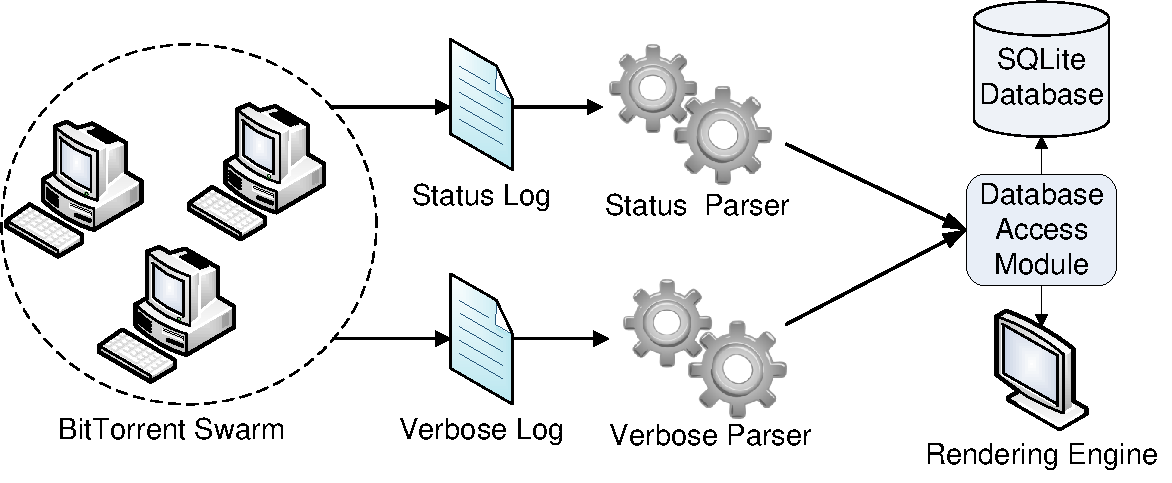
\includegraphics[width=0.7\textwidth]{src/img/proto-measure/logarch-not-use}
  \end{center}
  \caption{Logging System Overview}
  \label{fig:proto-measure:logarch}
\end{figure}

As shown in Figure~\ref{fig:proto-measure:logarch}, using parsers specific to
each type of logging file, messages are sent as input to the \textit{Database
Access} module that stores them into an SQLite database. In order to analyse
peer behaviour, the \textit{Rendering Engine} reads stored logging data using
the \textit{Database Access} module and outputs it to a graphical user
interface.

\subsection{Post Processing Framework for Real-Time Log Analysis}

The dubbed post processing framework is used for storing logging information
provided by various BitTorrent clients into a storage area (commonly a
database). An architectural view of the framework is described in
Figure~\ref{fig:proto-measure:ppf-architecture}.

\begin{figure}[h]
  \begin{center}
    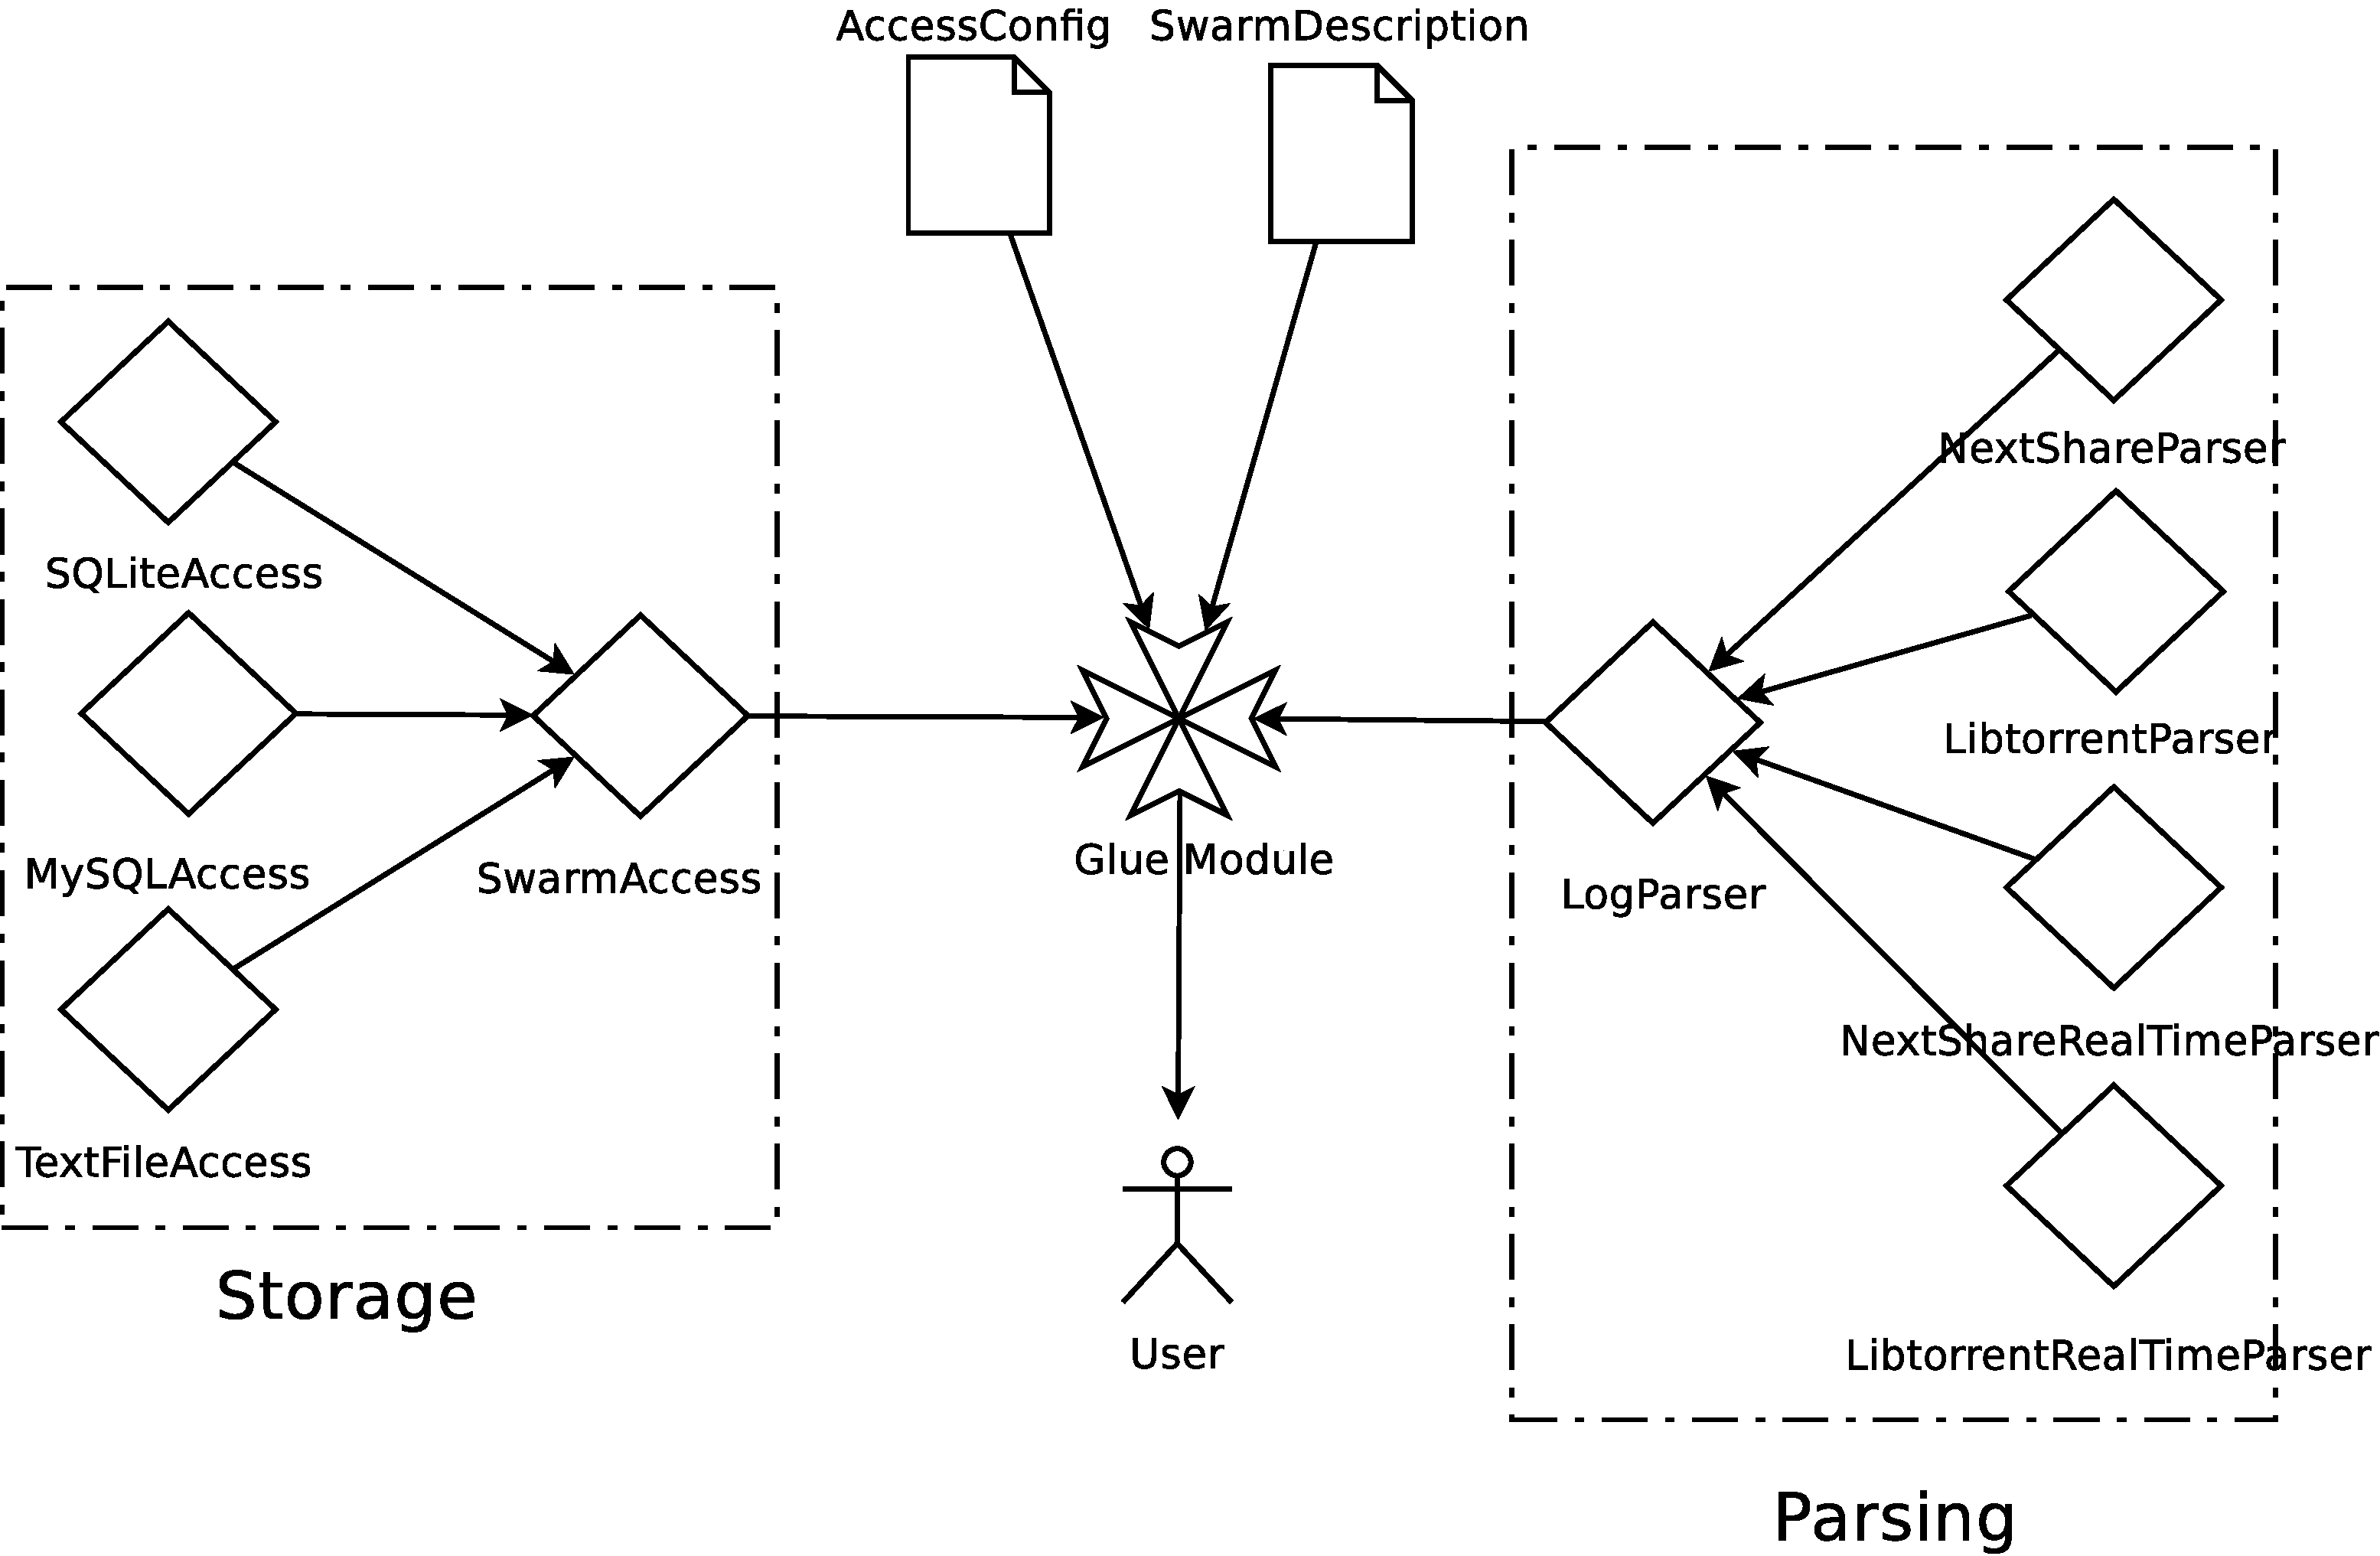
\includegraphics[width=0.7\textwidth]{src/img/proto-measure/ppf-architecture}
  \end{center}
  \caption{Post-Processing Framework Architecture}
  \label{fig:proto-measure:ppf-architecture}
\end{figure}

The two main components of the framework are the parser and the storage
components. Parsers process log information and extract measured protocol
parameters to be subject to analysis; storers provide an interface for
database or file storing -- both for writing and reading. Storers thus provide
an easy to access, rapid to retrieve and extensible interface to parameters.
Storers are invoked when parsing messages -- for storing parameters, and when
analyzing parameters -- for retrieving/reading/accessing parameters.

Client monitoring is enabled through the use of
MonALISA\footnote{\url{http://monalisa.cern.ch/monalisa.htm}}. MonALISA-specific
scripts are used to provide required information to the central repository.
The script is typically invoked every 5 seconds. The service station collects
required information and sends them to the monitoring repository.

\section{Evaluation Based on Peer-to-Peer Protocol Measurements}
\label{sec:proto-measure:eval-swarm}

The virtualized infrastructure and automated framework provides the necessary
platform for experimental evaluation of Peer-to-Peer implementations and
formal models. Our interest resides in evaluating BitTorrent clients, which
mostly translates to sheer download speed; the higher the download speed, the
better the performance. Obviously, we have to take into account both peer
download speed and swarm download speed. A peer with high download speed that
more or less ``free rides'' on top of the other peers is not desired in a
given swarm.

In order to properly consider a formal evaluation mechanism for performance
evaluation of a Peer-to-Peer ecosystem, several questions must be answered:

We will consider download speed
as an evaluation unit for performance. We consider the other measurable unit
to correlate to the download speed.

The varying units influence the measured units. Though we will focus mostly on
download speed, the other units also provide influence. If a given peer
receives a boost in its upload speed that means it will also boost download
speed of sever other peers. If a given varying unit would directly influence
upload speed, that will also provide influence over download speed, though it
may not happen directly. It may be easier to detect influence of varying units
over secondary units, such as protocol messages.

As such, we consider a correspondence between varying units and measured
units:

\begin{align}
\label{eq:proto-measure:eval}
Eval(hw, sys, impl, swarm, net) = (protomsg, speed, conn, ruse)
\end{align}

Our goal is to maximize download speed translates in defining and/or adjusting
the most suitable values for the varying units. A proper implementation,
deployed in a proper environment will ensure increased performance.

If we were to continuously monitor download speed, a pure mathematical formula
for a given peer would be:

\begin{align}
  FS = \int_0^{DT} DS(t)\,dt
\end{align}

where:

\begin{itemize}
  \item FS -- file size
  \item DT -- download time
  \item DS -- download speed (evolution)
\end{itemize}

As we only periodically monitor a peer, the formula translates to:

\begin{align}
  FS = \sum_{t=0}^{DT} DS_{t}
\end{align}

This provides necessary correlation between download speed evolution and
download time, with the file size being well known.

In order to correlate download speed with other units, we have to consider
download speed as the interaction with other peers. A peer may only download
if other peers upload. We formalize this as a download matrix that may
be built for each interval of monitoring:

\begin{align}
  PDS_{t} =
  \begin{pmatrix}
    ds_{1,1} = 0 & ds_{1,2} & \cdots & ds_{1,NP} \\
    ds_{2,1} & ds_{2,2} = 0 & \cdots & ds_{2,NP} \\
    \vdots & \vdots & \ddots & \vdots \\
    ds_{NP,1} & ds_{NP,2} & \cdots & ds_{NP,NP} = 0 \\
  \end{pmatrix}
\end{align}

where:

\begin{itemize}
  \item $ds_{i,j}$ -- download speed of peer \texttt{j} from peer \texttt{i};
  \item \texttt{PDS} -- peer download speed matrix at time \texttt{t};
  \item \texttt{NP} -- number of peers in swarm;
\end{itemize}

It follows that the upload matrix is the transpose of the download matrix. The
download speed of peer $j$ from peer $i$ ($ds_{i,j}$) is equal to the upload
speed of peer $i$ from peer $j$ ($us_{j,i}$). That is:

\begin{align}
  PUS_{t} = PDS_{t}^{T}
\end{align}

The instant download speed of a peer is the sum of all download speeds of peer
transfers. Similarly, the instant upload speed of a peer is the sum of all
upload speeds of peer transfers. In other words, the instant download speed of
peer $k$ ($DS_{k}$) is the sum of items in column $k$ in the $PDS$ matrix,
while the instant upload speed of peer $k$ ($US_{k}$) is the sum of items in
row $k$ in the $PDS$ matrix. That is:

\begin{align}
  DS_{k} = \sum_{i=1}^{NP} ds_{i,k}
\end{align}
\begin{align}
  US_{k} = \sum_{i=1}^{NP} ds_{k,i}
\end{align}

Please take into account that the matrix is a reporting tool. It does not
provide any configuration option for the functioning of a swarm; it is a
read-only database that is updated as the swarm evolves. Evolution of peers
and swarm is made possible by peer interaction, network connections, network
bandwidth availability and limitation; these are the action points that have
to be updated/enhanced; the matrix will subsequently provide reporting
information.

Consider the ideal situation of a swarm where:

\begin{itemize}
  \item The transferred file size is $FS$.
  \item There are $NP$ peers in the swarm.
  \item All peers have equal bandwidth $B$.
  \item Bandwidth is shared equally among peer connections.
  \item There is only one seeder (consider the case of live streaming).
  \item All peers start at the same time.
\end{itemize}

In this situation, all peer connections use $\frac{B}{NP}$ -- this is the
download speed and upload speed among any two peers. In the ideal
situation, the seeder sends piece 1 to peer 1, piece 2 to peer 2 and so on
(considering the bandwidth usage). In the next round it would send piece 1+NP
to peer 1, piece 2+NP to peer 2 and so on. In this round, all peers would
connect to each other and deliver the piece they have to the other peers and
receive their piece in return. That is, at the end of each round, all peers
(except for the seeder) have the same data -- in a full mesh network.

As such all peers fully use their bandwidth; all connections to other peers
are fully utilized. That means that the matrix is filled with the value
$\frac{B}{NP}$, except for the first column (the seeder download column) filled
with zeros. As such, the peer download speed is:

\begin{align}
  DS_{k} = \sum_{i=1}^{NP} \frac{B}{NP} = B
\end{align}

The file size formula for all peers is thus equal to:

\begin{align}
  FS = \sum_{i=1}^{DT} B
\end{align}

It follows that the download time is:

\begin{align}
  DT = \frac{FS}{B}
\end{align}

However, one has to consider the upload slot limitation of each peer.
Consider $NS$ the number of upload slots of each peer. In order to create a
full mesh network such as the one above, only $NS+1$ peers have to be present
(one of which is considered the seeder). For these peers, it results in the
same download time as above:

\begin{align}
  DT = \frac{FS}{B}
\end{align}

The next stage uses each previous seeder as a leecher. That is $(NS+1) \times
NS$ new leechers will get the full file. In the next phase, $((NS+1) \times
NS+1) \times NS$ new leechers will get the full file and so one.

The above approach poses two important disadvantages. Firstly, not all peers
receive content from the very beginning, which is problematic for streaming.
Secondly, it provides a high turnaround time, that is peers completing their
download later on.

An alternate approach is using an empty slot in the initial peers. When
seeder is started pieces are sent to $NS$ peers. Those peers use only $NS-1$
slots, since they are unable to provide anything to the seeder. The empty slot
may be used to provide data to another peer. That is there will be another
$NS$ peers that will be on round behind that will receive all pieces delivered
by the seeder in the previous round. This goes on until all peers receive
information. Such that, the download time would be:

\begin{itemize}
  \item For the first $NS$ peers: $DT = \frac{FS}{B}$
  \item For the next $NS$ peers: $DT = \frac{FS}{B} + t$
  \item For the next $NS$ peers: $DT = \frac{FS}{B} + 2t$
  \item And so on.
\end{itemize}

$t$ is the time required for transferring one piece or item of the file. This
approach is highly adequate for streaming, allows a good turnaround time and
is also highly similar to the BitTorrent swarm model allowing interactions
with many other peers. The model has its limitations, in not mentioning peer
arrival time, the fact that ``upper'' peers are benevolent seeders for
``lower'' peers and the unchanged bandwidth among peers.
